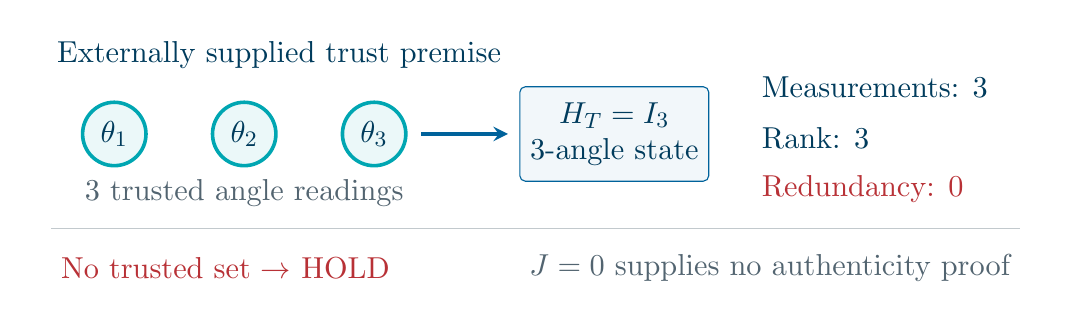
\begin{tikzpicture}[x=1cm,y=1cm,font=\fontsize{11}{13}\selectfont,>=stealth]
\definecolor{IEEEBlue}{HTML}{00629B}
\definecolor{Cyan}{HTML}{00A6B2}
\definecolor{Navy}{HTML}{003B5C}
\definecolor{Slate}{HTML}{526470}
\definecolor{CaseRed}{HTML}{B83136}
\path[use as bounding box] (0,0) rectangle (13,3.5);
\node[anchor=west,text=Navy] at (.25,3.16) {Externally supplied trust premise};
\foreach \x/\n in {1.1/1,2.75/2,4.4/3} {
  \node[circle,draw=Cyan,line width=1.3pt,fill=Cyan!8,minimum size=.7cm,text=Navy] (s\n) at (\x,2.15) {$\theta_{\n}$};
}
\node[text=Slate] at (2.75,1.4) {3 trusted angle readings};
\draw[->,IEEEBlue,line width=1.3pt] (5,2.15)--(6.1,2.15);
\node[draw=IEEEBlue,fill=IEEEBlue!5,rounded corners=2pt,minimum width=2.4cm,minimum height=1.2cm,align=center,text=Navy] at (7.45,2.15) {$H_T=I_3$\\3-angle state};
\node[anchor=west,text=Navy] at (9.2,2.75) {Measurements: 3};
\node[anchor=west,text=Navy] at (9.2,2.1) {Rank: 3};
\node[anchor=west,text=CaseRed] at (9.2,1.45) {Redundancy: 0};
\draw[Slate!35] (.3,.95)--(12.6,.95);
\node[anchor=west,text=CaseRed] at (.3,.45) {No trusted set $\rightarrow$ HOLD};
\node[anchor=east,text=Slate] at (12.6,.45) {$J=0$ supplies no authenticity proof};
\end{tikzpicture}%
